\documentclass[tikz,border=4pt]{standalone}
% Estilo común de los diagramas de bloques (se usa con \input en cada standalone)
\usepackage[defaultsans,scale=0.92]{lato}
\usepackage{libertinust1math}
\usepackage{xcolor,amsmath}
\usepackage{tikz}
\usetikzlibrary{positioning,arrows.meta,calc,shapes.geometric}
\usepackage{../../notacion}
\definecolor{ctrlazul}{HTML}{1E5AA8}\definecolor{ctrlnoche}{HTML}{14213D}
\definecolor{ctrlcoral}{HTML}{D1495B}\definecolor{ctrlverde}{HTML}{2A9D8F}
\definecolor{ctrlambar}{HTML}{E09F3E}\definecolor{ctrlgris}{HTML}{5C677D}
\definecolor{ctrlvioleta}{HTML}{6C4AB6}\definecolor{ctrlteal}{HTML}{0F7173}
\tikzset{
  >={Stealth[length=2.4mm]}, every node/.style={font=\small},
  bloque/.style={draw=ctrlnoche,fill=ctrlazul!7,thick,rounded corners=1.5pt,minimum height=9mm,minimum width=13mm,inner sep=4pt},
  suma/.style={draw=ctrlnoche,thick,circle,inner sep=0pt,minimum size=6mm},
  senal/.style={->,thick,draw=ctrlnoche},
  rot/.style={font=\footnotesize,text=ctrlgris},
}

\usetikzlibrary{decorations.pathmorphing}
\begin{document}
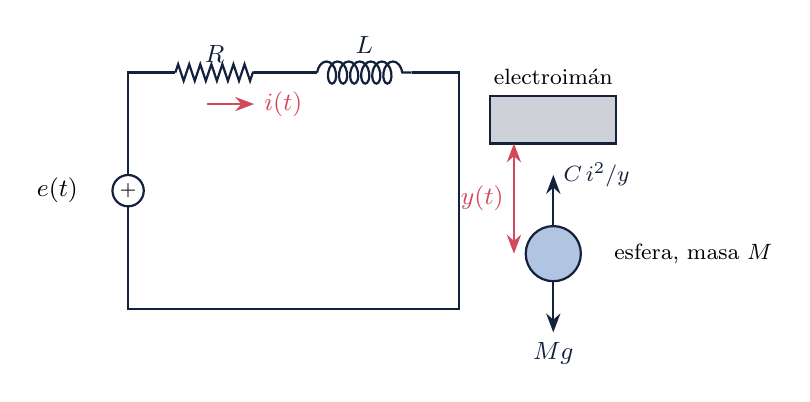
\begin{tikzpicture}[font=\small]
  \draw[thick,ctrlnoche] (0,0) node[circle,draw,thick,fill=white,inner sep=4pt] (fu) {} ;
  \node at (0,0) {\scriptsize$+$}; \node[left=3mm of fu] {$e(t)$};
  \draw[thick,ctrlnoche] (fu.north)--(0,1.5)--(0.6,1.5);
  \draw[thick,ctrlnoche,decorate,decoration={zigzag,segment length=4pt,amplitude=3pt}] (0.6,1.5)--(1.6,1.5) node[midway,above]{$R$};
  \draw[thick,ctrlnoche] (1.6,1.5)--(2.4,1.5);
  \draw[thick,ctrlnoche,decorate,decoration={coil,aspect=0.6,segment length=4pt,amplitude=4pt}] (2.4,1.5)--(3.6,1.5) node[midway,above=3pt]{$L$};
  \draw[thick,ctrlnoche] (3.6,1.5)--(4.2,1.5)--(4.2,-1.5)--(0,-1.5)--(fu.south);
  \draw[->,thick,ctrlcoral] (1.0,1.1)--(1.6,1.1) node[right]{$i(t)$};
  \draw[thick,ctrlnoche,fill=ctrlgris!30] (4.6,0.6) rectangle (6.2,1.2); \node[font=\footnotesize] at (5.4,1.45) {electroimán};
  \draw[thick,ctrlnoche,fill=ctrlazul!35] (5.4,-0.8) circle (0.35); \node[right=3mm,font=\footnotesize] at (5.75,-0.8) {esfera, masa $M$};
  \draw[<->,ctrlcoral,thick] (4.9,0.6)--(4.9,-0.8) node[midway,left]{$y(t)$};
  \draw[->,thick,ctrlnoche] (5.4,-1.15)--(5.4,-1.8) node[below]{$Mg$};
  \draw[->,thick,ctrlnoche] (5.4,-0.45)--(5.4,0.2) node[right,font=\footnotesize]{$C\,i^2/y$};
\end{tikzpicture}
\end{document}
